\chapter{UPPAAL and Formal Verification}
\section{Property Verification}
UPPALL has its own query language used to verify properties of a model\cite[p. 7]{upptut}. The language is a simplified version of timed computation tree logic. UPPAAL's query language consists of \textit{state formulae} and \textit{path formulae}. The path formulae can be categorised into three categories: reachability, safety and liveness. These are described below, and they are summarised in \cref{fig:query}.
\paragraph{State formulae}
A state formula is an expression which can be evaluated for a state, without looking at the mode, e.g. $i \geq 42$. This formula asks whether it is true that $i$ is greater than or equal to $42$ in a given state. State formulae also allow one to verify whether a process is in a given location using an expression of the form \texttt{P.l}, where \texttt{P} is a process and \texttt{l} is a location in the process.\\\\
%deadlock special case
A deadlock is described using a special state formula, \texttt{deadlock}, and is satisfied for all states which deadlock.
\paragraph{Reachability properties} express the notion that a state formula, $\varphi$, can \textit{possibly} be satisfied on some path, going from the initial location of the model. In UPPAAL it is expressed as \texttt{E<>$\varphi$}. This could for example be used to verify whether a variable \texttt{i} in the model, along some path going from the initial location will have the value $2$ by querying the model with \texttt{E<>i == 2}.\\\\
These types of properties are often verified as a part of a sanity check of a modelled system\cite[p. 8]{upptut}. For example, when modelling Java bytecode, one can verify that the program will reach the end state, at some point. Though this does not give any guarantee that the program will always finish, it makes sense to make sure to check whether it possibly \textit{can}.
\ch{improve clarity}
\paragraph{Safety properties} state that ``something bad will never happen''. In other words, every state in a model will invariantly satisfy $\varphi$. This is useful e.g. to check that a bit flip can not cause a modelled program to end up in a location where e.g. incorrect credentials are authenticated and subsequently approved. Such an invariant safety property is expressed in UPPAAL as \texttt{A[]$\varphi$}, where the state formula, $\varphi$, would express that the simulation of the model would never end up in the approved location when the credentials are incorrect.\\\\
A variant of this safety property, is one that expresses that ``something will possibly never happen'', e.g. when playing a game, a safe state would be one where a winning move is always possible. This is expressed in UPPAAL as \texttt{E[]$\varphi$}, which states that there should exist a maximal path\footnote{A maximal path, is a path that is either infinite or the last state has no outgoing edges that can be traversed.}, where $\varphi$ is always true.
\paragraph{Liveness property} state that ``something will eventually happen''. This could for example be that when a coffee maker is turned on, it will eventually output coffee. It is expressed in UPPAAL as \texttt{A<>$\varphi$}, and means that $\varphi$ is eventually satisfied.\\\\
A variation of this liveness property, is the \textit{leads to} property, written as $\varphi \leadsto \psi$. It is expressed in a UPPAAL query as \texttt{$\varphi$ --> $\psi$}, and means that if $\varphi$ is satisfied, $\psi$ will eventually be satisfied, e.g. whenever a message has been sent, it will eventually be received.

\begin{figure}
\centering
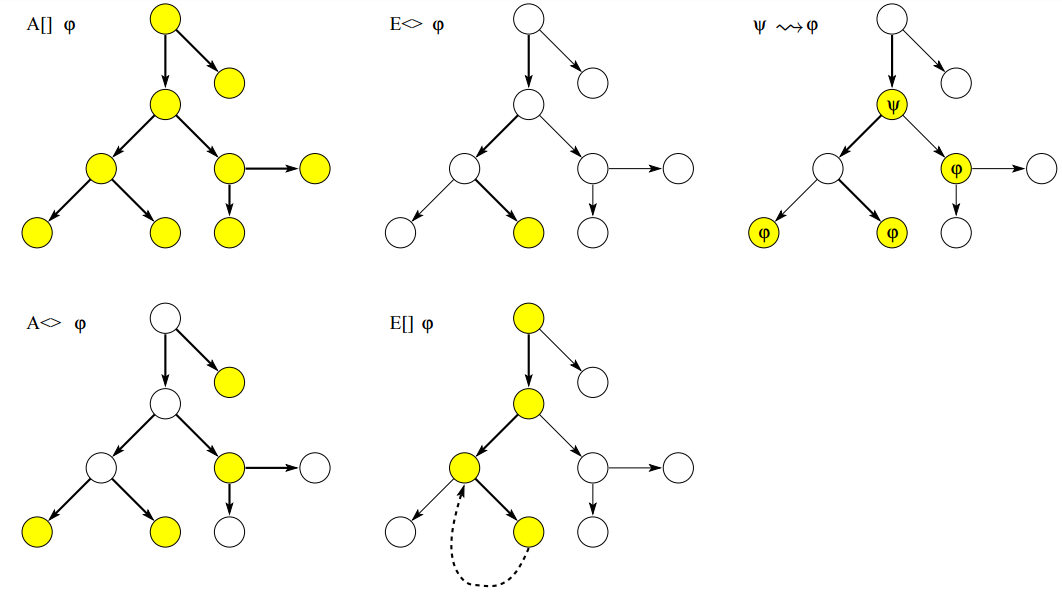
\includegraphics[width=0.9\textwidth]{queries.png}
\caption{Illustration of the different property verification queries in UPPAAL. Taken from \cite[p. 8]{upptut}}.
\label{fig:query}
\end{figure}

\section{SMC}
extra edges for waiting